\chapter{Úvod}\label{chap:intro}

Tejto úvodnej kapitole by som vás chcel trochu oboznámiť s mojou bakalárkou a poukázať na moju východziu situáciu. Ďalej tiež platformy na ktorých beží a prečo.
\section{Vysvetlenie názvu}
Moja bakalárka sa volá \uv{Optimalizácia obchodovacieho algoritmu na vysoko volatilných komoditných burzách}. Najprv by som tento názov rozobral a podrobne vysvetlil čo to znamená.
\subsection{Optimalizácia obchodného algoritmu}
Vyvíjame algoritmus ktorý bude vedieť sám obchodovať. Mojou úlohou bude tento algoritmus testovať a následne optimalizovať aby podával čo najlepšie výsledky.
\subsection{Vysoko volatilných}
Volatilita\cite{Volatilita} je kolísanie. Miera neistoty. A investíciám je vlastná. Platí, že čím vyššie výnosy, tým vyššia volatilita. Z toho vychádza aj pravidlo investičného horizontu, ktorý je pri rizikovejších – teda volatilnejších – aktívach dlhší. Prečo hľadáme  vysoko volatilné burzy ukážem na príklade.
\subsection{Komoditných burzách}
Náš algoritmus bude pracovať na komoditných burzách konkrétne na burzách pseudo-mien hlavne bitcoin. 

\section{Prečo volatilných?}
Tejto časti sa zameriam na okrajové burzy ktoré sú špecifické svojou vysokou volatilitou
a ukážeme výhody a nevýhody okrajových búrz. A nakoniec zhrnieme prečo nám vyhovujú práve okrajové burzy.
\subsection{Výhody}
\subsubsection{Vysoká volatilita}
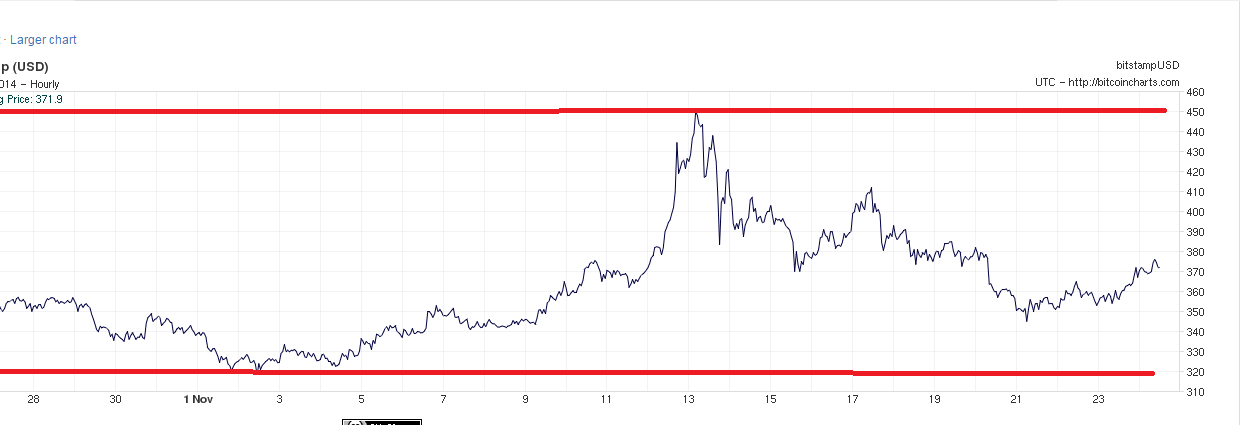
\includegraphics[width=1\textwidth]{obr}
Toto je príklad keď pozeráme na vysoko volatilnú burzu ktorou je bitcoin a USD. Možný zisk sa pohybuje až na úrovni 37.5 percenta keď nerátame poplatky. V prvom obrázku je jeden dielik 10 dolárov. 
\\
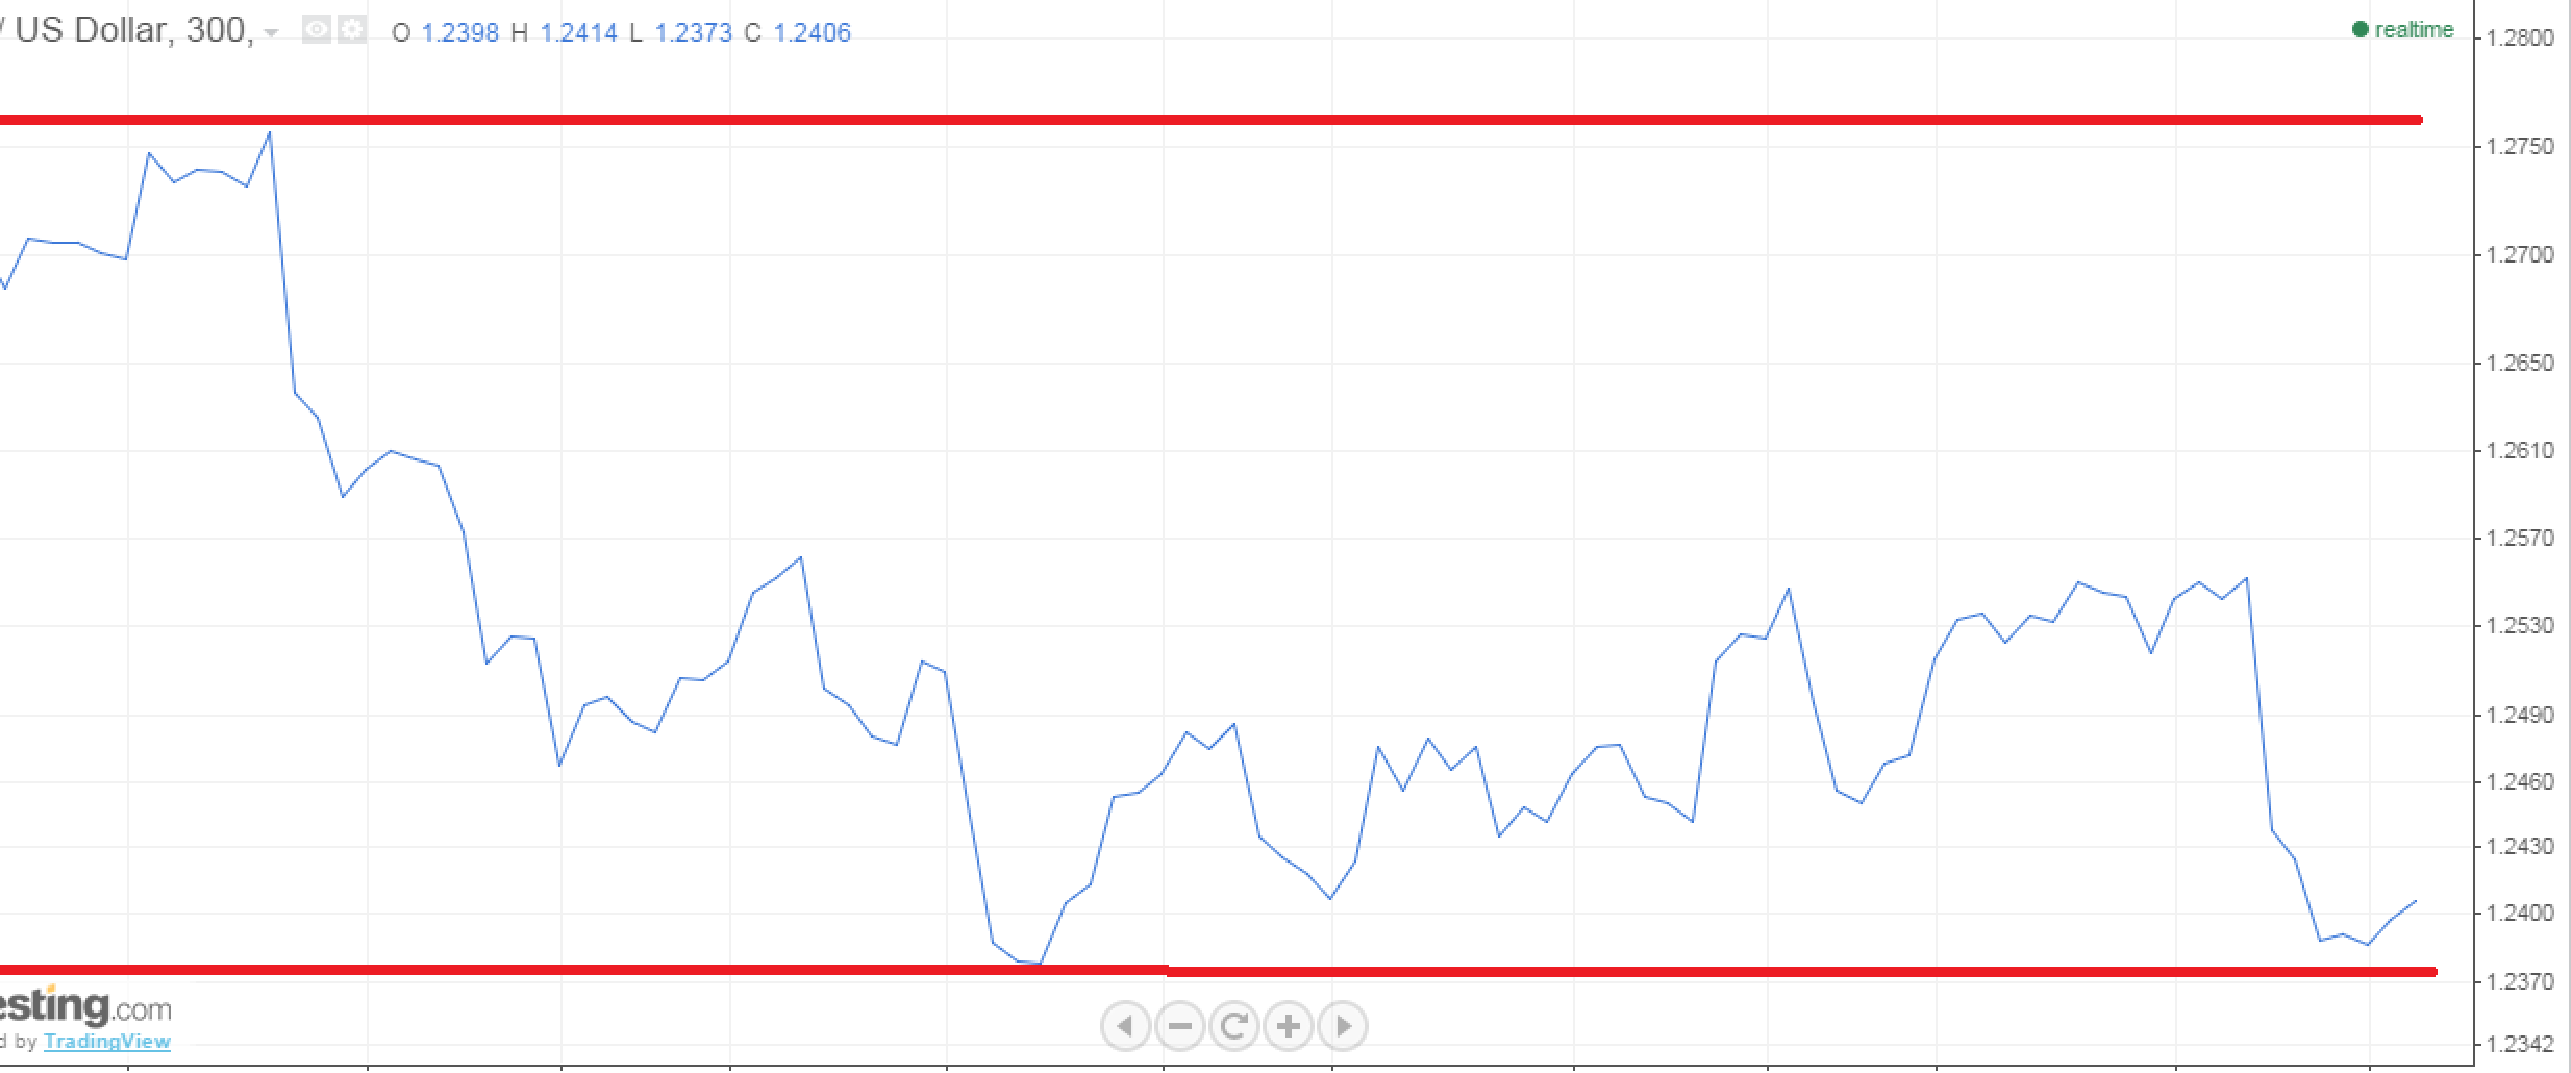
\includegraphics[width=1\textwidth]{obr2}
Na rozdiel od ďalšej málo volatilnej burzy kde je  možný zisk iba 2.95 percenta a jeden dielik je tisícina danej meny.
\subsubsection{Absencia \uv{Veľkých hráčov}}
Veľký hráči\cite{ZAC} sú hlavne veľké korporácie a bohatý investori. Za to my sme na trhu malí hráči lebo 
máme malí kapitál. A prečo nie sú na okrajových burzách veľký hráči? Práve preto lebo na okrajových burzách sa točí malé množstvo peňazí a na ich investíciách by sa výrazne prejavila likvidita čo vysvetlím v nevýhodách.
\subsubsection{Malé vstupné poplatky}
Keďže máme malí kapitál ktorý investujeme, veľmi rýchlo by sme skrachovali, keby sme robili často obchody čo veľakrát treba. Takže veľkou výhodou na okrajových burzách je že sa dajú nájsť burzy s minimálnymi vstupnými a inými poplatkami.
\subsection{Nevýhody}
\subsubsection{Veľká likvidita}
Najprv vysvetlím pojem \uv{spread}
\subsubsection{Väčšie riziko}
